\documentclass[12pt,a4paper,twoside,openright]{book}

\usepackage[USenglish,english]{babel}
\usepackage[utf8]{inputenc}

\usepackage{style/isi_style_lt}

\usepackage{amsmath,amsfonts,amssymb,amsthm}
\usepackage{caption}
\usepackage[usenames]{color}
\usepackage{enumerate}
\usepackage{fancyhdr}
\usepackage{fancyvrb}
\usepackage{float}
\usepackage{graphicx}
\usepackage{indentfirst}
\usepackage{listings}
\usepackage{marvosym}
\usepackage{multicol}
\usepackage{sectsty}
\usepackage{subcaption}
\usepackage{tocloft}
\usepackage[table]{xcolor}
\usepackage{url}
\usepackage{multirow}

\AtBeginDocument{%
	\renewcommand{\contentsname}{Table of contents}
	\renewcommand\tablename{Table}
	\renewcommand\figurename{Figure}
	\renewcommand{\lstlistingname}{List}
	\renewcommand{\refname}{Ref.}
}

\definecolor{dkgreen}{rgb}{0,0.6,0}
\definecolor{gray}{rgb}{0.5,0.5,0.5}
\definecolor{mauve}{rgb}{0.58,0,0.82}

\lstset{
  frame=single,
  captionpos=b,
  language=Java,
  aboveskip=3mm,
  belowskip=3mm,
  showstringspaces=false,
  columns=flexible,
  basicstyle={\small\ttfamily},
  numbers=none,
  numberstyle=\tiny\color{gray},
  keywordstyle=\color{blue},
  commentstyle=\color{dkgreen},
  stringstyle=\color{mauve},
  breaklines=true,
  breakatwhitespace=true,
  tabsize=3
}

\makeatletter
\def\cleardoublepage{
	\clearpage\if@twoside \ifodd\c@page\else
	\hbox{}
	\thispagestyle{empty}
	\newpage
	\if@twocolumn\hbox{}\newpage\fi\fi\fi
}

\makeatother

\setlength{\textwidth}{14cm}
\setlength{\textheight}{21cm}
\setlength{\footskip}{3cm}

\setlength{\hoffset}{0pt}
\setlength{\voffset}{0pt}

\setlength{\oddsidemargin}{1cm}
\setlength{\evensidemargin}{1cm}

\universita{Alma Mater Studiorum -- Università di Bologna}

\campus{Campus di Cesena}

\scuola{Scuola di Ingegneria e Architettura}

\corsodilaurea{Laurea Magistrale in Ingegneria e Scienze Informatiche}

\titolo{Used Cars Analysis}

\materia{Big Data}

\laureando{Gabriele Guerrini}

\annoaccademico{2019 -- 2020}

\makeindex

\begin{document}

\frontmatter 

\maketitle

\tableofcontents

\mainmatter

\pagestyle{fancy} 
\fancyhead[LE,RO]{\thepage}
\fancyfoot{}

\chapter{Dataset and query}

\section{Dataset}

The dataset can be downloaded at: 

\bigskip

\begin{center}
  \textbf{https://www.kaggle.com/austinreese/craigslist-carstrucks-data}.
\end{center}

\bigskip

It contains data about more than 400k used cars for sale in US.
Each car is described by several info such as price, odometer, manufacturer, year, sale region and so on.

\section{Query}

\subsection{Description}

The query to be executed is the following one:

\bigskip

``For each region, it must be found the OPI of the most widespread brand in such region, considering cars that use gas fuel only. 

OPI is an acronym for Odometer-Price Index and represents the average ratio odometer/price. It is calculated upon all cars of a given brand in the country, regardless of other car features (fuel type, number of cylinders...).''

\newpage
\subsection{Workflow}\label{workflow}

Figure \ref{fig:MR-workflow} shows the adopted workflow\footnote{It is not the optimal one since the same query could be executed in less than four job. The idea is to structure the workflow this way so that few different algorithms (e.g. filtering, projection, summarization, join) and optimizations (e.g. caching) can be applied. }.

The pipeline is made up of four different jobs, that is:
\begin{itemize}
  \item \textbf{Job 1: Preprocessing}: It executes all preprocessing operation needed to correctly use the dataset in next jobs. Firstly, it cleans the raw dataset by droppinig records that contain missing values and by eliminating useless columns. Then, it executes the dataset growth operation, namely, each remaining record is copied by a certain replication factor so that the output dataset contains enough amount of data. The default replication factor is 100.  
  \item \textbf{Job 2a: Opi}: It calculates the OPI for each brand.
  \item \textbf{Job 2b: Region}: It calculates the most widespread brand for each region.
  \item \textbf{Job 3: Join}: It merges partial results of jobs 2a and 2b.
\end{itemize}

\begin{figure}[H]
	\centering
	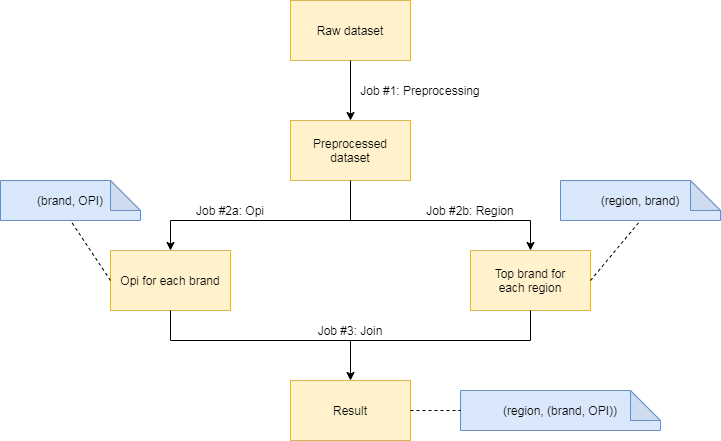
\includegraphics[scale=0.6]{images/2-mapreduce/MR-workflow.png}
	\caption{Adopted workflow for query execution.}
	\label{fig:MR-workflow}
\end{figure}

%The dataset cardinality is reduced from 423858 to 231157 * replicationFactor.
%The dataset size is reduced from 1GB to 8.2MB * replicationFactor.



\chapter{MapReduce}

\section{Jobs}

\subsection{Job 1: Preprocessing}

Job execution and interfaces are described in figure \ref{fig:MR-job-1}.
 
Each raw record is read and parsed into a ``Car'', i.e. a custom ``Writable'' object, during map stage. 
Each ``Car'' stores data about:
\begin{itemize}
 \item Region
 \item Price
 \item Brand
 \item Fuel
 \item Odometer
\end{itemize}

The mapper output is a pair where the key is the default one used by Hadoop when reading text files and the value is the ``Car'' itself.

The reduce stage replaces the default key with a ``NullableWritable'' so that the whole job output is a set of records yet. Then, it publishes each record several times as specified by the replication factor.

\begin{figure}[H]
	\centering
	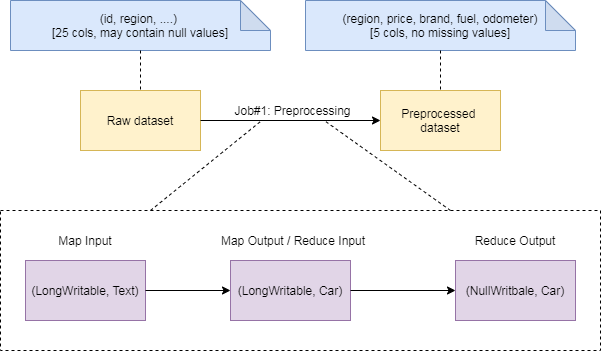
\includegraphics[scale=0.7]{images/2-mapreduce/MR-job-1.png}
	\caption{Description of ``job 1: preprocessing'' workflow and interfaces.}
	\label{fig:MR-job-1}
\end{figure}

\subsection{Job 2a: Opi}

Job execution and interfaces are described in figure \ref{fig:MR-job-2a}.

The map stage input value is a ``Car'' encoded as text. The key is the Hadoop default one (it won't be used). The mapper calculates the OPI for a given car using price and odometer fields and gives a pair consisting of (brand, OPI) as output.

The reduce stage just calculates average values using single OPIs and reports it as output.
   
\begin{figure}[H]
	\centering
	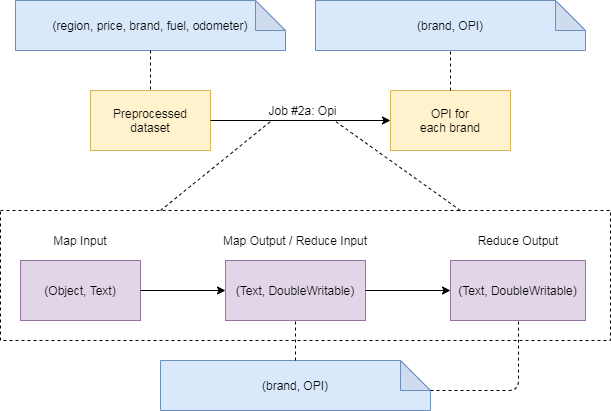
\includegraphics[scale=0.7]{images/2-mapreduce/MR-job-2a.png}
	\caption{Description of ``job 2a: opi'' workflow and interfaces.}
	\label{fig:MR-job-2a}
\end{figure}  

\subsection{Job 2b: Region}

Job execution and interfaces are described in figure \ref{fig:MR-job-2b}.

The map stage input value is a ``Car' encoded as text. The key is the Hadoop default one for text files (it won't be used). If the fuel type is correct, the mapper generates as output a pair (region, brand) so that reduce stage can operate per region basis.

The reducer, given a region, firstly calculates the cardinality for each brand by collecting the input pairs. Then, it calculates the maximum and gives it as output in the form of (region, brand).

\begin{figure}[H]
	\centering
	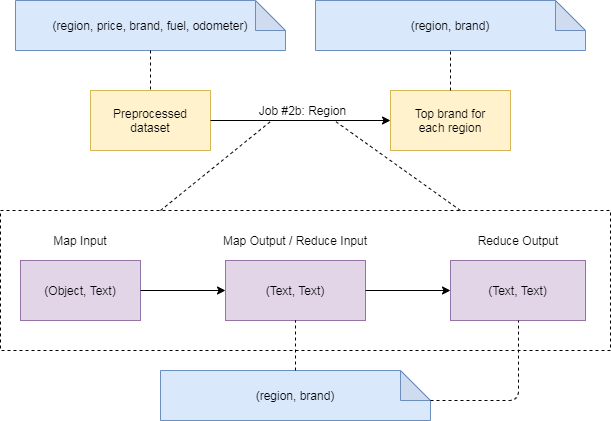
\includegraphics[scale=0.7]{images/2-mapreduce/MR-job-2b.png}
	\caption{Description of ``job 2b: region'' workflow and interfaces.}
	\label{fig:MR-job-2b}
\end{figure}  

\subsection{Job 3: Join}

Job execution and interfaces are described in figure \ref{fig:MR-job-3}.

The map stage takes as input pairs structured as (Text, Text). The source of a given pair can be from job 2a output or from job 2b output. By examinating it, it is discovered the source and the pair is marked with a flag.
Since the join key will be the brand, the output of map stage is a pair (brand, (flag, region)), where flag and region are encapsulated into a ``JoinPair'' (a custom ``Writable'').

The reducer executes the join algorithm on input items and creates output pairs in the form (region, (brand, OPI)). 

\begin{figure}[H]
	\centering
	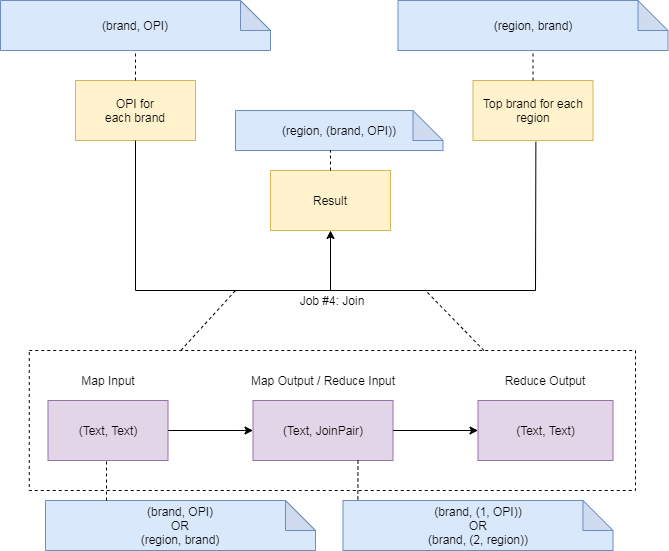
\includegraphics[scale=0.7]{images/2-mapreduce/MR-job-3.png}
	\caption{Description of ``job 3: join'' workflow and interfaces.}
	\label{fig:MR-job-3}
\end{figure}  


\section{Performance evaluation}

Performance are evaluated by varying the number of reducers, by enabling the use of combiners and by considering different replication factors.

Each casuistry result is the average value upon 3 runs. Results are shown in tables \ref{table-mr-perf-1} and \ref{table-mr-perf-100}.

As we can notice, the optimal number of reducers is 5\footnote{Actually, a more fine-grained analysis could be done by tuning the number of reducers on sigle jobs (instead of the same for each one). This could lead to find a more efficint setup but the number of combinations is quite huge and this argument will not be covered. }: too many reducers are an overkill due to task bootstrap and to the slender amount of data; on the other hand, too few reducers can't parallelize the work in the best way.  

\begin{table}[H]
  \centering
  \begin{tabular}{ |c c|c c c c c c c| } 
    \hline
    \multicolumn{2}{ |c| }{} & \multicolumn{7}{ c| }{Reducers} \\
    \multicolumn{2}{ |c| }{} & 1 & 2 & 5 & 6 & 8 & 10 & 100 \\
    \hline
    \multirow{2}{4em}{Combiner} 
    & No  & 292 & 244 & 223 & 235 & 251 & 280 & 1235 \\      
    & Yes &  &  &  &  &  &  & \\ 
    \hline
  \end{tabular}
  \caption{Performance results expressed as elapsed time in seconds using \textbf{replication factor = 100}.}
  \label{table-mr-perf-100}
\end{table}

\begin{table}[H]
  \centering
  \begin{tabular}{ |c c|c c c c c| } 
    \hline
    \multicolumn{2}{ |c| }{} & \multicolumn{5}{ c| }{Reducers} \\
    \multicolumn{2}{ |c| }{} & 1 & 2& 5& 10 & 100 \\
    \hline
    \multirow{2}{4em}{Combiner} 
    & No  & 223 & 162 & 168 & 216 & 1400 \\      
    & Yes &  &  &  &  &   \\ 
    \hline
  \end{tabular}
  \caption{Performance results expressed as elapsed time in seconds using \textbf{replication factor = 1}.}
  \label{table-mr-perf-1}
\end{table}
\chapter{Spark}

\section{Job description}

A unique Spark file will execute all jobs specified in section \ref{workflow}. The dataset is loaded as a Spark ``DataFrame'' and every operation will lean on ``SparkSQL'' layer.

Figure \ref{fig:spark-DAG} shows the complete DAG corresponding to the main job created by Spark. Figure \ref{fig:spark-DAG-info} shows Spark DAG accompained with few extra info.

\newpage
\begin{figure}[H]
	\centering
	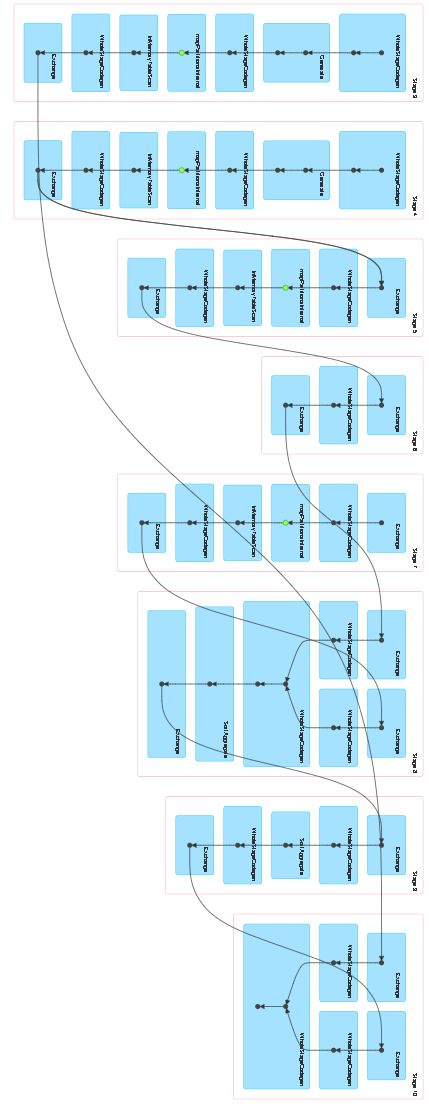
\includegraphics[scale=0.8]{images/3-spark/spark-DAG.png}
	\caption{Complete Spark DAG.}
	\label{fig:spark-DAG}
\end{figure}

\begin{figure}[H]
	\centering
	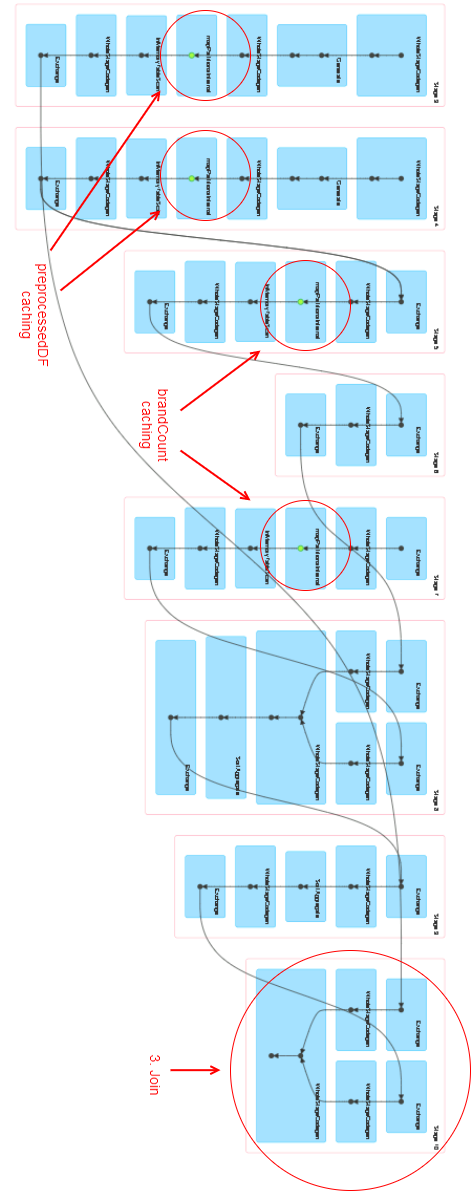
\includegraphics[scale=0.8]{images/3-spark/spark-DAG-info.png}
	\caption{Extra info about Spark DAG.}
	\label{fig:spark-DAG-info}
\end{figure}

Since the size of tables used in the two join operations is not excessive, the usage of the broadcast feature may be used on one table. Such an operation makes Spark split the job in three pipelined different jobs (few stages are skipped though).

The broadcast version results on an overall of 800 tasks (against the 1200 of the basic one), a more efficient usage of memory (garbage collection time) and a decrease of execution time close to 8/9\%.

DAGs for the broadcast version are reported in figures \ref{fig:sspark-broad-DAG-1}, \ref{fig:spark-broad-DAG-2} and \ref{fig:spark-broad-DAG-3}.

\begin{figure}[H]
	\centering
	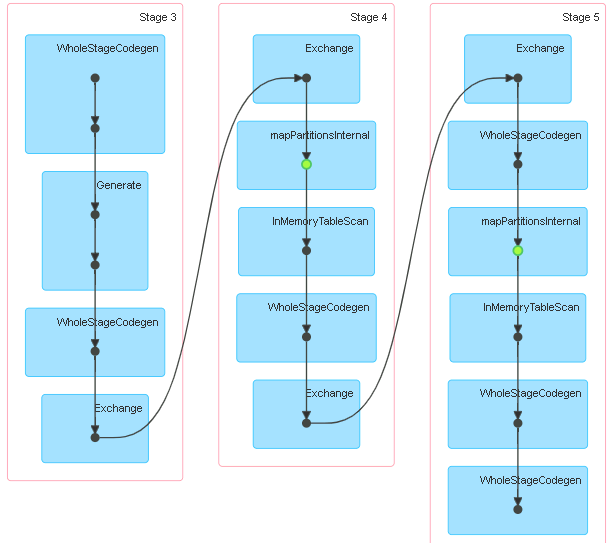
\includegraphics[scale=0.8]{images/3-spark/broad-DAG-1.png}
	\caption{DAG for first job created by Spark when using broadcast on join.}
	\label{fig:sspark-broad-DAG-1}
\end{figure}


\begin{figure}[H]
	\centering
	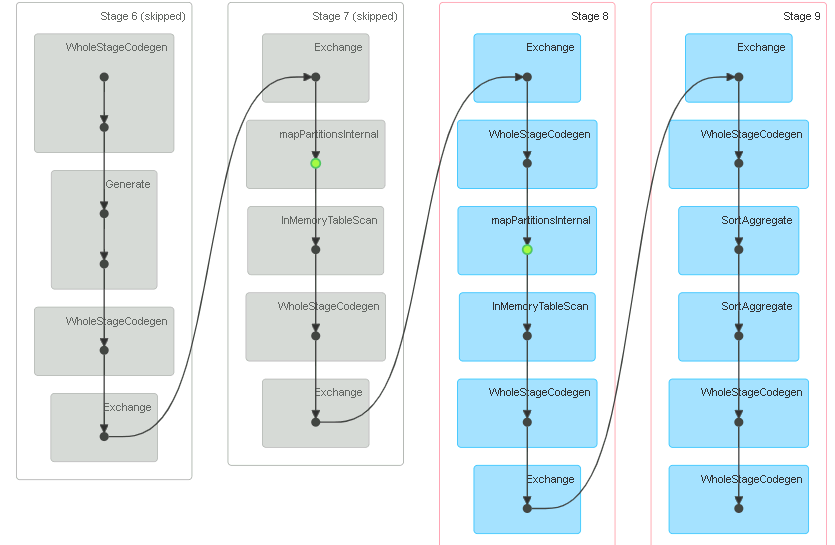
\includegraphics[scale=0.65]{images/3-spark/broad-DAG-2.png}
	\caption{DAG for second job created by Spark when using broadcast on join.}
	\label{fig:spark-broad-DAG-2}
\end{figure}


\begin{figure}[H]
	\centering
	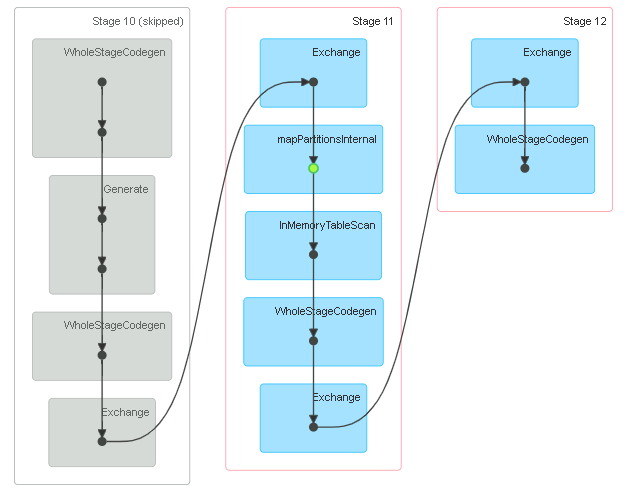
\includegraphics[scale=0.65]{images/3-spark/broad-DAG-3.png}
	\caption{DAG for third job created by Spark when using broadcast on join.}
	\label{fig:spark-broad-DAG-3}
\end{figure}


\section{Performance evaluation}

Performance are evaluated by varying the number of executors and cores per executor. 

Let's consider cluster characteristics (10 nodes, 4 cores per node) and given constraints (usage of 8 CPUs at most).   
Each casuistry result is the average value upon 3 runs. Results are shown in table \ref{table:spark-perf}.

As we can notice, results confirm common best practice rules: best performances among all more promising combinations are obtained using the maximum amount of resources (8 CPUs); moreover, the whole application speeds up when assigning more than one core to each executor.

\begin{table}[H]
  \centering
  \begin{tabular}{ |c c|c c c c c| } 
    \hline
    \multicolumn{2}{ |c| }{} & \multicolumn{5}{ c| }{Executors} \\
    \multicolumn{2}{ |c| }{} & 1 & 2 & 3 & 4 & 8 \\
    \hline
    \multirow{3}{4em}{Cores per executor} 
    & 1 &  &    &    &    & 88 \\      
    & 2 &  &    & 94 & 79 & \\ 
    & 3 &  & 96 &    &    & \\     
    \hline
  \end{tabular}
  \caption{Performance results expressed as elapsed time in seconds using \textbf{replication factor = 100} for most promising combinations.}
  \label{table:spark-perf}
\end{table}



\chapter{Conclusions}

As it could be foreshadowed, empirical results confirm theorical results and common best practice rules, that is:
\begin{itemize}
  \item \textit{MR vs Spark}: by using best setup found for both programs, Spark (60s ca.) performs better than MR (210s ca.). 
  \item \textit{Architecture overkill}: It is confirmed that architecture based on cluster, HDFS, Hadoop and so on are designed to work with huge amount of data. Indeed, by varying replication factor, the cluster scales wery well. Rather, such an architecture results to be an overkill for small datasets.
  \item \textit{MR reducers and combiners}: Optimal number of reducers makes sense if considering number of nodes and amount of data; moreover, the usage of combiners in right points can improve performances. 
  \item \text{Spark executors}: number of executors and core assigned to each one follow common best practice rules when considering available resources and cluster characteristics.
\end{itemize}
	
\backmatter	

\end{document}